\documentclass[aspectratio=169]{beamer} % 16:9 aspect ratio
\usepackage{capt-of}
% --- THEME AND COLOR ---
\usetheme{Madrid} % A popular, clean theme with a sidebar
% Other good themes: CambridgeUS, Boadilla, Warsaw, Singapore
\usecolortheme{dolphin} % A decent color theme that works well with Madrid
% Other color themes: dolphin, whale, orchid

% --- PACKAGES ---
\usepackage[utf8]{inputenc}
\usepackage[T1]{fontenc}
\usepackage{amsmath}
\usepackage{amssymb}
\usepackage{graphicx}
\usepackage{booktabs} % For nice tables (if needed)
\usepackage{hyperref} % For links (usually Beamer handles this)
\usepackage{textcomp} % For \textdegree C etc.
\usepackage{lmodern} % Or any other nice font package
\usepackage[colorlinks=true,linkcolor=blue,urlcolor=blue]{hyperref}

% --- PRESENTATION METADATA ---
\title[Eulerian Two-Fluid Simulations]{Eulerian Two-Fluid Simulations of Gas-Solid Flows in Fluidized Bed}
\subtitle{M.Tech. Project CLD880}
\author[Sajeev Shyam]{Sajeev Shyam (2021CH70457) \\ Supervisor: Prof. Vivek Buwa}

\institute[2021CH70457]{
    Department of Chemical Engineering, IIT Delhi\\
}
\date{May 2025} % Or use \date{\today} for the presentation date

% --- IIT DELHI LOGO ---
% You'll need to upload an image named 'iitd_logo.png' to your Overleaf project
\titlegraphic{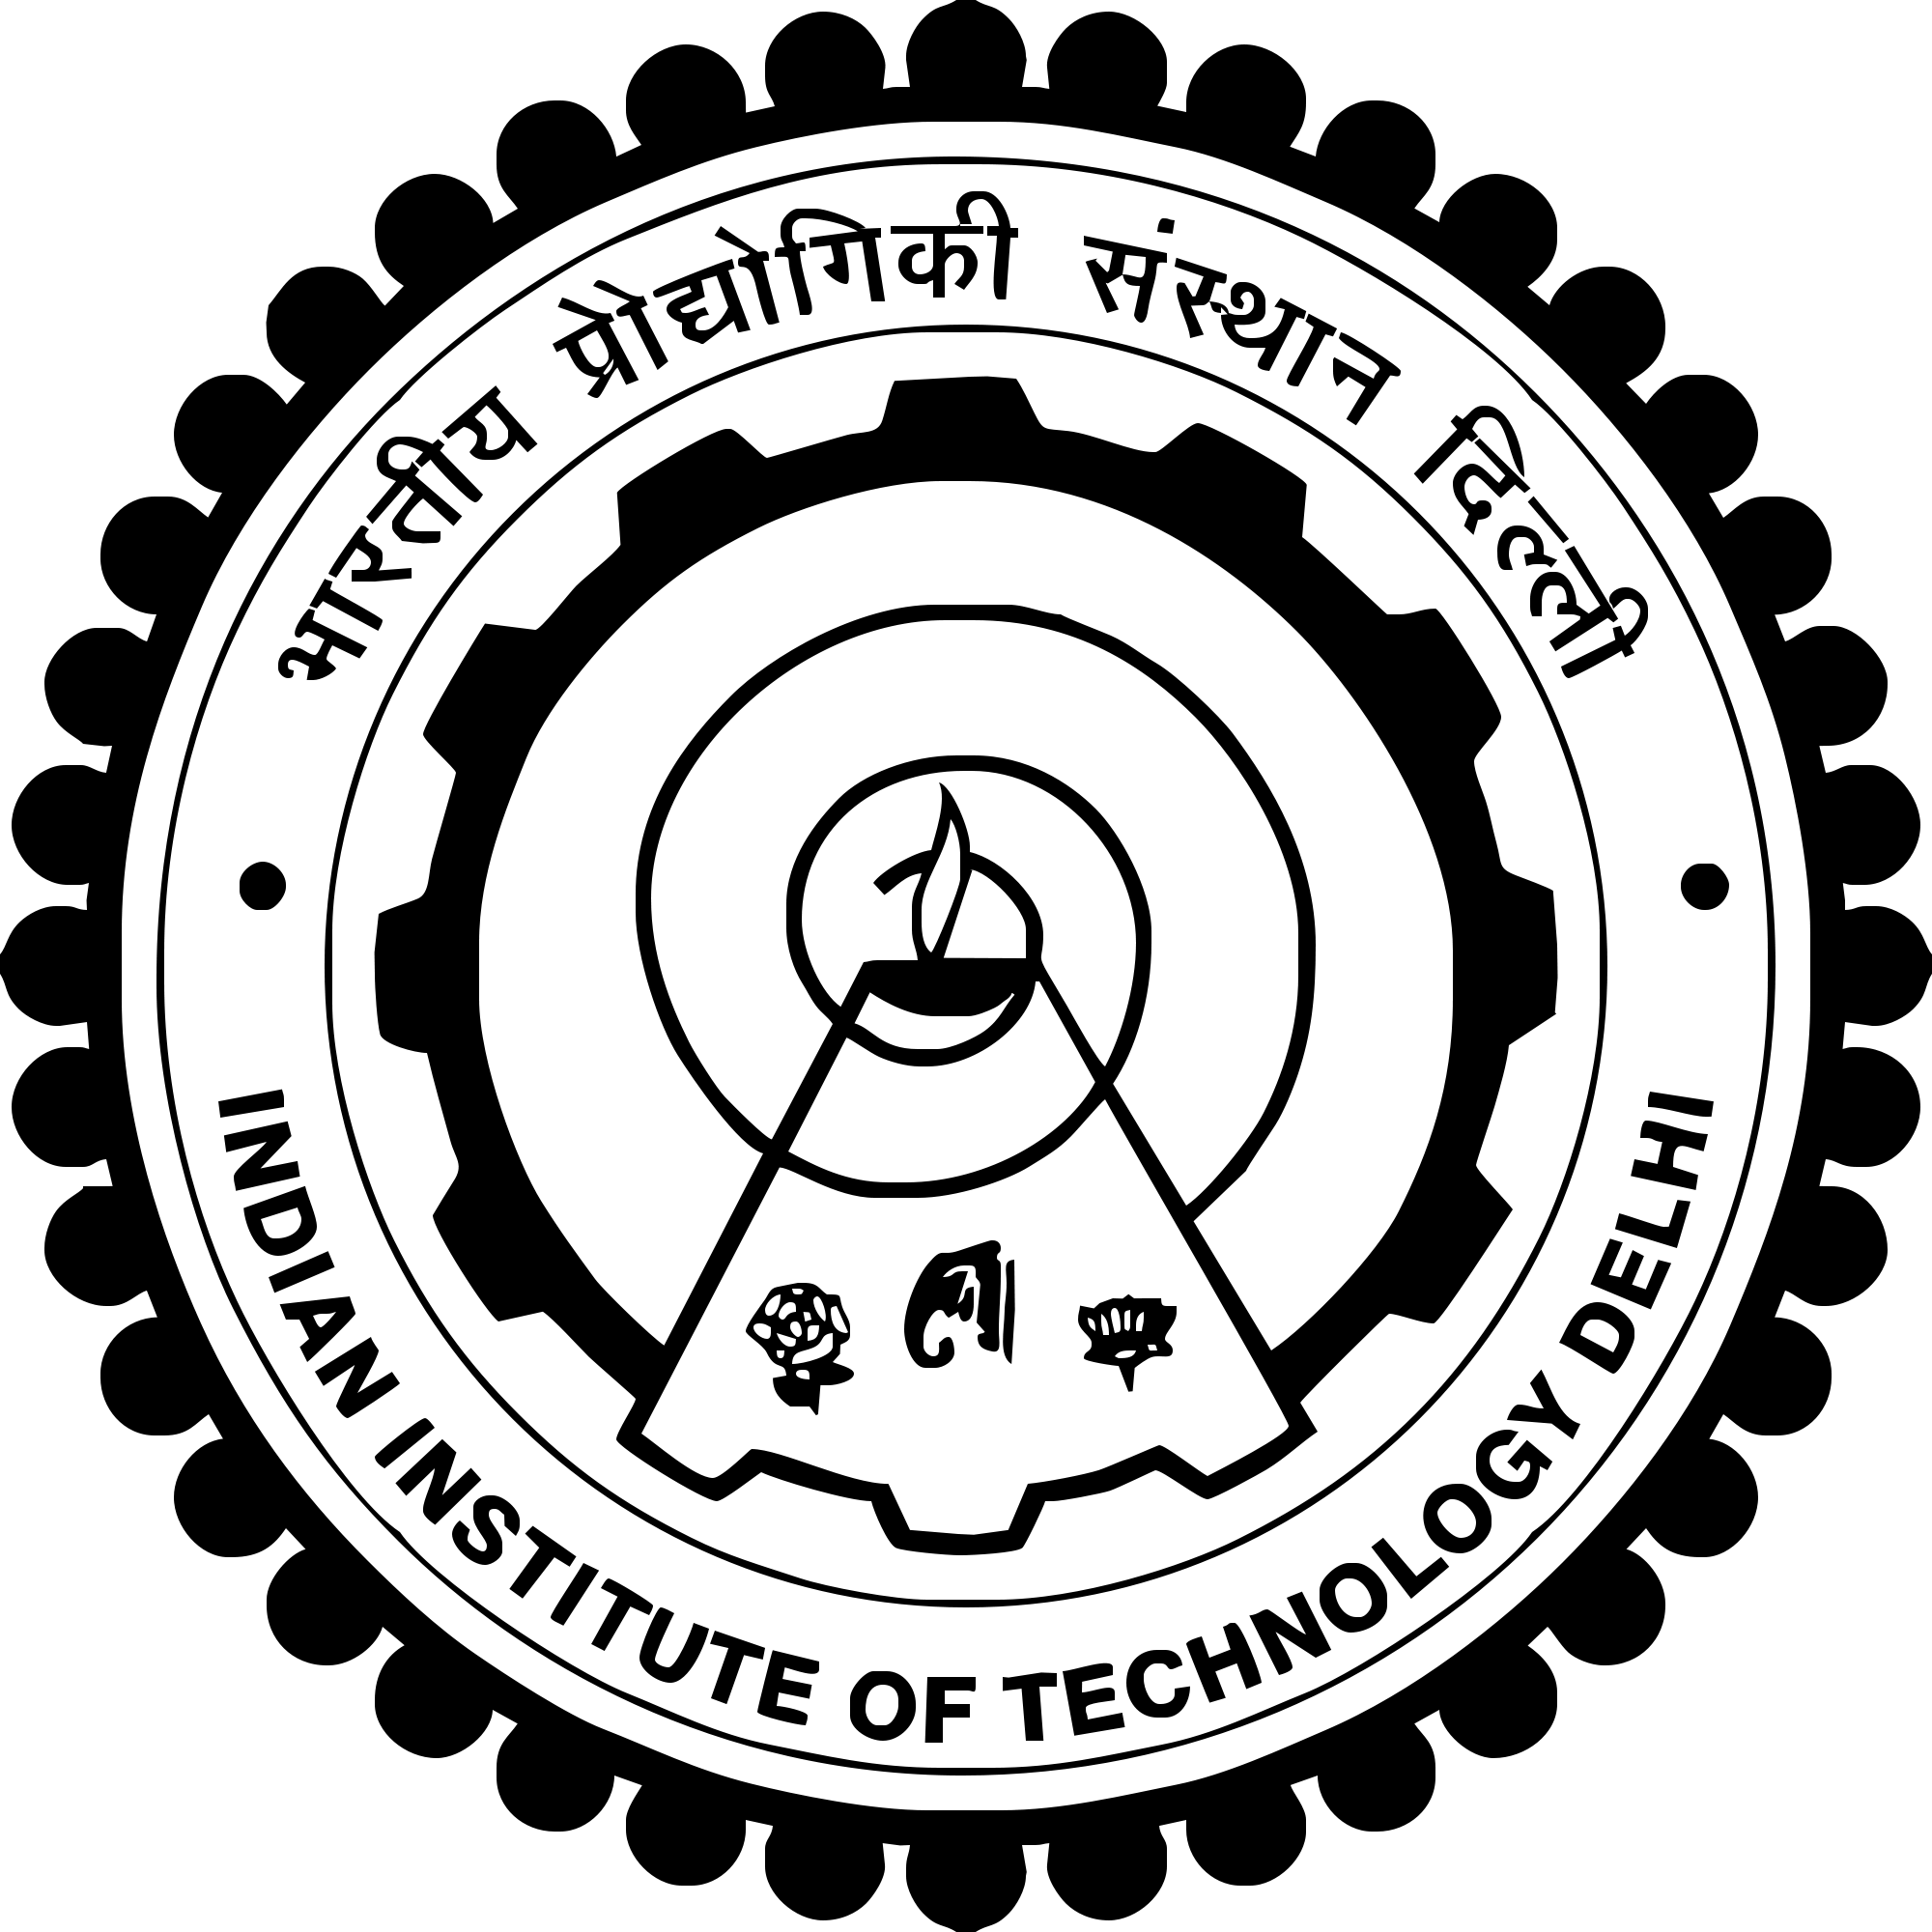
\includegraphics[width=2cm]{iitd_logo.png}} % Adjust width as needed

% --- COMMANDS FOR EASIER BULLET POINTS ---
\newcommand{\bi}{\begin{itemize}}
\newcommand{\ei}{\end{itemize}}
\newcommand{\ben}{\begin{enumerate}}
\newcommand{\een}{\end{enumerate}}
\newcommand{\im}{\item}
\makeatletter
% Solution to center the footline title relative to the main content area
% for themes like Madrid with a sidebar.
\defbeamertemplate*{footline}{madridcustomcenter}
{
  \leavevmode%
  \hbox{%
  % Box 1 (Author/Institute): Width is 1/3 of paperwidth + half of sidebar width
  % This makes it extend further into the main content area from the left.
  \begin{beamercolorbox}[wd=\dimexpr\paperwidth/3 + 0.5\sidebarwidth\relax,ht=2.25ex,dp=1ex,center]{author in head/foot}%
    \usebeamerfont{author in head/foot}\insertshortauthor~~(\insertshortinstitute)
  \end{beamercolorbox}%
  % Box 2 (Title): Width remains 1/3 of paperwidth.
  % Its *position* is now shifted right because Box 1 is wider.
  % The center of this box will align with the center of the main content area.
  \begin{beamercolorbox}[wd=\dimexpr\paperwidth/3\relax,ht=2.25ex,dp=1ex,center]{title in head/foot}%
    \usebeamerfont{title in head/foot}\insertshorttitle
  \end{beamercolorbox}%
  % Box 3 (Date/Pagenumber): Width is 1/3 of paperwidth - half of sidebar width.
  % This makes it narrower to accommodate the shift.
  \begin{beamercolorbox}[wd=\dimexpr\paperwidth/3 - 0.5\sidebarwidth\relax,ht=2.25ex,dp=1ex,right]{date in head/foot}%
    \usebeamerfont{date in head/foot}\insertshortdate{}\hspace*{2em}%
    \insertframenumber{} / \inserttotalframenumber\hspace*{2ex}%
  \end{beamercolorbox}}%
  \vskip0pt%
}
% Apply the custom footline
\setbeamertemplate{footline}[madridcustomcenter]
\makeatother
\setbeamertemplate{navigation symbols}{}

\begin{document}

% --- TITLE PAGE ---
\begin{frame}
    \maketitle
\end{frame}

% --- INTRODUCTION ---
\section{Introduction}
\begin{frame}{Introduction: Fluidization \& FBRs}
    \begin{columns}[T] % Top-align columns
        \begin{column}{0.7\textwidth}
            \begin{block}{Fluidization}
                \bi
                    \im Transition of granular solid material into a liquid-like state.
                    \im Achieved by upward fluid flow counteracting particle weight.
                    \im Bed expands, particles suspend, exhibiting collective motion.
                    \im Blends characteristics of packed beds and mixed reactors (Kunii \& Levenspiel, 1991).
                \ei
            \end{block}
            \vspace{0.5em}
            \begin{block}{Fluidized Bed Reactors (FBRs)}
                \bi
                    \im Excellent heat and mass transfer characteristics.
                    \im Minimized concentration/temperature gradients.
                    \im Applications: Catalytic cracking, polymerization, combustion, gasification.
                \ei
            \end{block}
        \end{column}
        \begin{column}{0.3\textwidth}
            \centering
            % Keeping placeholder_fbr_schematic.png unless you provide a specific image for this
            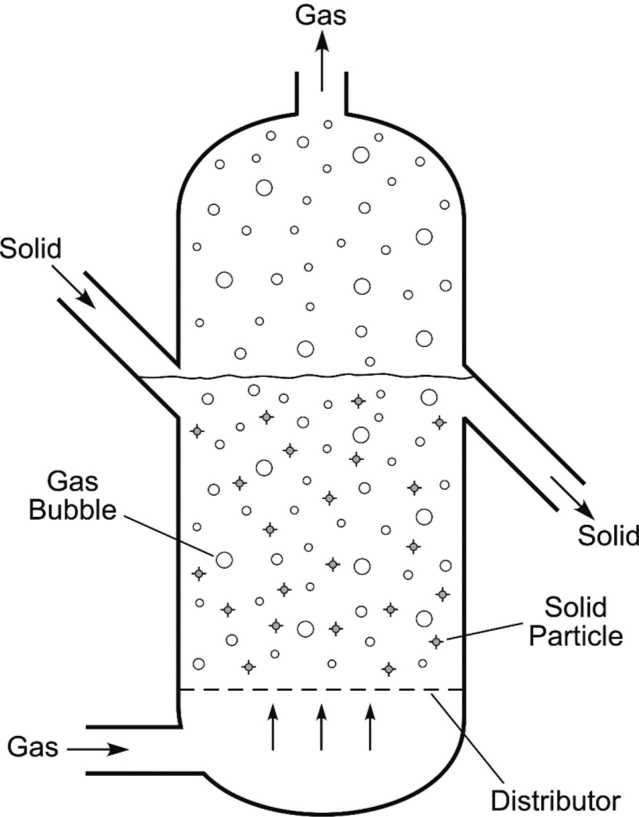
\includegraphics[width=\linewidth,height=1\textheight,keepaspectratio]{fludized_bed.png}\\ % MODIFIED HEIGHT
            \vspace{0.4em}
            {\tiny \caption{Schematic of a Fluidized Bed Reactor \\ \href{https://ebrary.net/131855/engineering/fluidized_reactor}{\underline {src: ebrary.net}}}}
        \end{column}
    \end{columns}
\end{frame}

\begin{frame}{Motivation \& CFD Approach}
    \begin{block}{Challenges in Modeling FBRs}
        \bi
            \im Complex hydrodynamics: incipient, bubbling, slugging, turbulent, circulating regimes.
            \im Multiphase nature: gas-solid interactions, turbulence, mesoscale structures.
            \im Experimental limitations in spatial/temporal resolution.
        \ei
    \end{block}
    \vspace{1em}
    \begin{block}{Computational Fluid Dynamics (CFD)}
        \bi
            \im Powerful tool for insights into bed hydrodynamics.
            \im Eulerian-Eulerian Two-Fluid Model (TFM): Phases as interpenetrating continua.
            \im Closures needed for interphase drag and granular stresses.
            \im This study: ANSYS Fluent, Kinetic Theory of Granular Flow (KTGF), Gidaspow drag model.
        \ei
    \end{block}
\end{frame}

% --- OBJECTIVES ---
\section{Objectives}
\begin{frame}{Objectives of This Study}
    \ben
        \im To develop and apply an Eulerian Two-Fluid Model (TFM) for simulating gas-solid fluidization in a pseudo-2D rectangular bed using ANSYS Fluent.
        \im To investigate the effect of superficial gas velocity on the hydrodynamic behavior, including:
            \ben
                \im Bubble formation and dynamics.
                \im Solids volume fraction distribution.
                \im Particle velocity patterns and circulation.
            \een
        % \im To understand the effect of mixture composition (mixtures of varying sizes and densities) on bubble formation dynamics for mono-dispersed particles.
    \een
    \vspace{1em}
\end{frame}

% --- THEORETICAL BACKGROUND ---
\section{Theoretical Background}
\begin{frame}{Eulerian-Eulerian Two-Fluid Model (TFM)}
    \begin{block}{Core Idea}
        Both gas (g) and solid (s) phases are treated as interpenetrating continua.
        Conservation equations are solved for each phase.
    \end{block}
    \vspace{-1.2em}
    \begin{columns}[T]
        \begin{column}{0.28\textwidth}
            \begin{block}{ \scriptsize Mass Conservation ($\alpha_g + \alpha_s = 1$)}
                Gas phase:
                \small
                \[ \frac{\partial}{\partial t}(\alpha_g \rho_g) + \nabla \cdot (\alpha_g \rho_g \vec{U}_g) = 0 \]
                Solid phase:
                \[ \frac{\partial}{\partial t}(\alpha_s \rho_s) + \nabla \cdot (\alpha_s \rho_s \vec{U}_s) = 0 \]
                {\tiny ($\alpha$: volume fraction, $\rho$: density, $\vec{U}$: velocity)}
            \end{block}
        \end{column}
        \begin{column}{0.68\textwidth}
            \begin{block}{\scriptsize Momentum Conservation }
                Gas phase:
                { \scriptsize
                \[ \frac{\partial}{\partial t}(\alpha_g \rho_g \vec{U}_g) + \nabla \cdot (\alpha_g \rho_g \vec{U}_g \vec{U}_g) = -\alpha_g \nabla P_g + \nabla \cdot \bar{\bar{\tau}}_g + \alpha_g \rho_g \vec{g} - \beta_{gs}(\vec{U}_g - \vec{U}_s) \] }
                Solid phase:
                {\scriptsize
                \[ \frac{\partial}{\partial t}(\alpha_s \rho_s \vec{U}_s) +  \nabla \cdot (\alpha_s \rho_s \vec{U}_s \vec{U}_s) = -\alpha_s \nabla P_g - \nabla P_s + \nabla \cdot \bar{\bar{\tau}}_s + \alpha_s \rho_s \vec{g} + \beta_{gs}(\vec{U}_g - \vec{U}_s) \]
                }
                \normalsize
                ($P_s$: solids pressure, $\bar{\bar{\tau}}$: stress tensor, $\beta_{gs}$: interphase drag)
            \end{block}
        \end{column}
    \end{columns}
\end{frame}

\begin{frame}{Closure Models}
    \begin{block}{Interphase Drag Coefficient ($\beta_{gs}$)}
        \bi
            \im Quantifies drag force between gas and particles.
            \im Depends on: particle size ($d_p$), gas properties ($\rho_g, \mu_g$), solids volume fraction ($\alpha_s$), relative velocity.
            \im \textbf{Gidaspow Model Used:} Blends Ergun equation (dense flow) and Wen-Yu model (dilute flow).
        \ei
    \end{block}
    \begin{block}{Kinetic Theory of Granular Flow (KTGF) for Solid Phase}
        Analogy to kinetic theory of gases to model particle interactions.
        \bi
            \im \textbf{Granular Temperature ($\Theta_s$):} Measure of random fluctuating kinetic energy of particles.
            \im \textbf{Solids Pressure ($P_s$):} Arises from particle collisions and contacts.
            \im \textbf{Solids Stress Tensor ($\bar{\bar{\tau}}_s$):} Represents internal friction/viscosity of granular flow. Derived from $\Theta_s$.
        \ei
    \end{block}
\end{frame}

\begin{frame}{Closure Models}
    \begin{block}{Wall Boundary Conditions}
        \bi
            \im Standard no-slip conditions are not suitable for particles.
            \im \textbf{Johnson \& Jackson Model Used:} Specifies slip velocity for solids at the wall, accounts for momentum and granular energy exchange during particle-wall collisions.
            \im Depends on specularity and restitution coefficients.
        \ei
    \end{block} 
\end{frame}

% --- MODELING SETUP ---
\section{Modeling Setup}
\begin{frame}{Geometry}
    \begin{columns}[T]
        \begin{column}{0.5\textwidth}
            \begin{block}{Computational Domain (Pseudo-2D)}
                \bi
                    \im Length (W, x-dir): 0.2 m
                    \im Depth (D, z-dir): 0.02 m (thin to approximate 2D)
                    \im Height (H, y-dir): 1.0 m
                    \im Solid Phase: 
                    \bi 
                        \im Inital Static bed height 0.2 m
                        \im Diameter: 2.26 mm
                    \ei
                \ei
            \end{block}            
        \end{column}
        \begin{column}{0.5\textwidth}
            \centering
            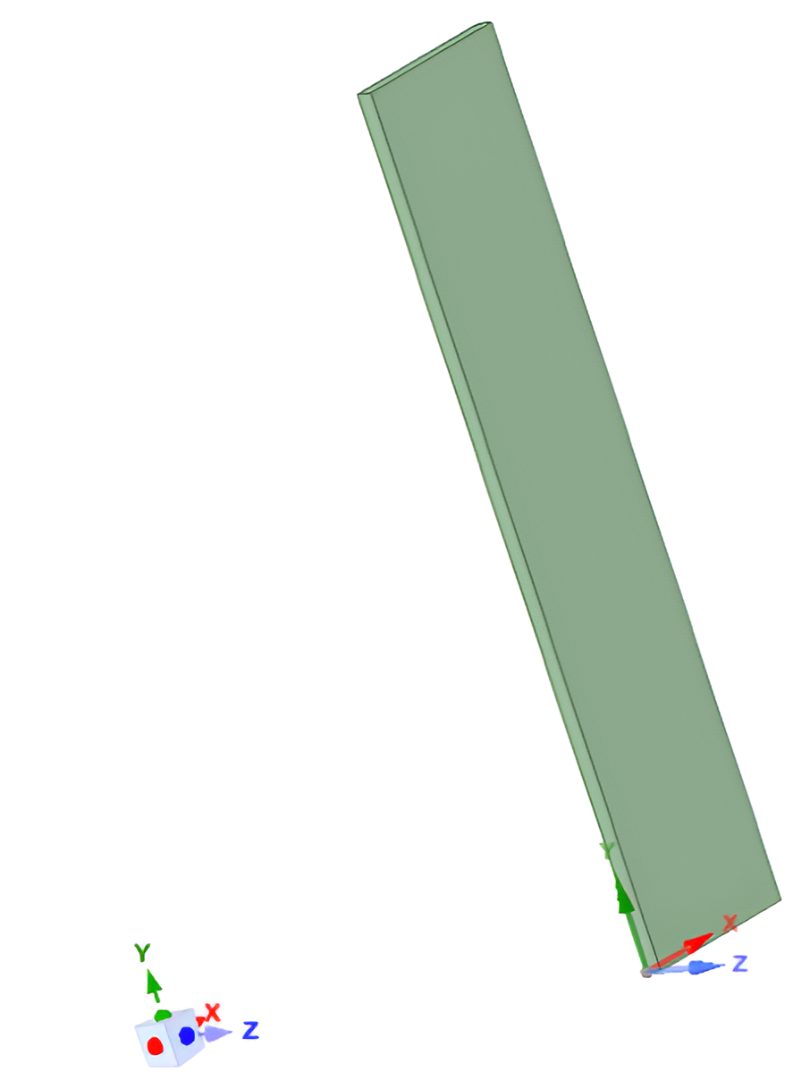
\includegraphics[width=0.8\linewidth,height=0.8\textheight,keepaspectratio]{geometry.png} \\ % MODIFIED HEIGHT
            \tiny Computational domain geometry
            \vspace{1em}
            
        \end{column}
    \end{columns}
\end{frame}

\begin{frame}{Meshing}
    \begin{columns}[T]
        \begin{column}{0.5\textwidth}
            \begin{block}{Meshing}
        \bi
            \im Uniform structured grid
            \im Divisions:
            \bi
                \im 70 in y-direction
                \im 20 in x-direction
                \im 4 in z-direction
            \ei
            \im Total cells: $70 \times 20 \times 4 = 5600$
        \ei
    \end{block}           
        \end{column}
        \begin{column}{0.5\textwidth}
            \centering
            
\includegraphics[width=0.8\linewidth,height=0.8\textheight,keepaspectratio]{mesh.png} \\
            \tiny Uniform structured grid            
        \end{column}
    \end{columns}
\end{frame}

% \begin{frame}{Computational Setup: Numerical Implementation}
%     \begin{block}{Solver & Core Model (ANSYS Fluent)}
%         \bi
%             \im Eulerian-Eulerian Two-Fluid Model (TFM)
%             \im Pressure-Velocity Coupling: Phase Coupled SIMPLE algorithm
%         \ei
%     \end{block}
%     \vspace{0.5em}
%     \begin{columns}[T]
%         \begin{column}{0.48\textwidth}
%             \begin{block}{Spatial Discretization Schemes}
%                 \bi
%                     \im \textbf{Gradient:} Green-Gauss Cell Based
%                     \im \textbf{Pressure:} PRESTO!
%                     \im \textbf{Momentum:} Second Order Upwind
%                     \im \textbf{Volume Fraction:} QUICK
%                     \im \textbf{Granular Temp.:} Second Order Upwind
%                 \ei
%             \end{block}
%         \end{column}
%         \begin{column}{0.48\textwidth}
%             \begin{block}{Temporal Discretization & Control}
%                 \bi
%                     \im \textbf{Scheme:} Second Order Implicit
%                     \im \textbf{Time Step ($\Delta t$):} 0.001 s
%                     \im \textbf{Max. Iterations/Step:} 40
%                     \im \textbf{Under-Relaxation:} Default values
%                 \ei
%             \end{block}
%         \end{column}
%     \end{columns}
% \end{frame}

\begin{frame}{Computational Setup: Domain Boundaries & Initial State}
    \begin{columns}[T]
        \begin{column}{0.48\textwidth}
            \begin{block}{Inlet Conditions (Bottom Boundary)}
                \textbf{Gas Phase (Velocity Inlet):}
                \bi
                    {\footnotesize \im Case 1 Superficial Velocity ($U_g$): 1.736 m/s
                    \im Case 2 Superficial Velocity ($U_g$): 2.78 m/s}
                \ei
                \vspace{0.3em}
                \textbf{Solid Phase:}
                \bi
                    \im Velocity: 0 m/s
                    \im Volume Fraction ($\alpha_s$): 0
                \ei
            \end{block}
            % \vspace{0.5em}
            \begin{block}{Outlet Condition (Top Boundary)}
                \bi
                    \im Type: Pressure Outlet
                    \im Gauge Pressure: 0 Pa
                \ei
            \end{block}
        \end{column}
        \begin{column}{0.48\textwidth}
            \begin{block}{Wall Conditions (Side, Front, Back)}
                \textbf{Gas Phase:}
                \bi
                    \im No-slip condition
                \ei
                \vspace{0.3em}
                \textbf{Solid Phase (Johnson-Jackson Model):}
                \bi
                    \im Specularity Coefficient: 0.05
                    \im Particle-Wall Restitution Coeff.: 0.9
                \ei
            \end{block}
            % \vspace{0.5em}
            \begin{block}{Initial Bed Configuration}
                Solid phase initially patched in the domain:
                \bi
                    \im Initial Bed Height: 0.2 m (20 cm)
                    \im Initial Solids Volume Fraction ($\alpha_s$): 0.6
                \ei
            \end{block}
        \end{column}
    \end{columns}
\end{frame}


\begin{frame}{Probe Location}
    \begin{columns}[T]
        \begin{column}{0.5\textwidth}
            \begin{block}{Probe for Time-Series Analysis}
                \begin{itemize}
                    \item A fixed point within the bed is monitored to record local, transient data.
                    \item Coordinates: (x, y, z) = (0.1 m, 0.1 m, 0.01 m)
                    \begin{itemize}
                        \item x = 0.1 m (center of width)
                        \item y = 0.1 m (above distributor, within initial bed height)
                        \item z = 0.01 m (center of depth)
                    \end{itemize}
                \end{itemize}
            \end{block}
        \end{column}
        \begin{column}{0.5\textwidth}
            \centering
            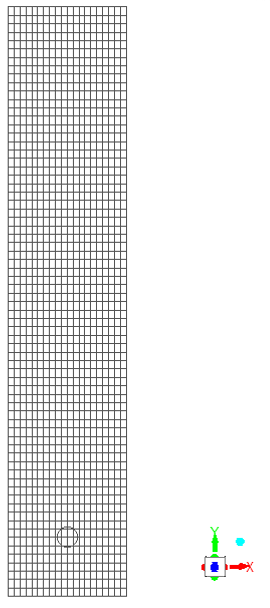
\includegraphics[width=0.75\textwidth,height=0.75\textheight,keepaspectratio]{probe_location_mesh.png} \\
            {\tiny Computational mesh showing probe location}
        \end{column}
    \end{columns}
\end{frame}

% --- RESULTS AND DISCUSSION ---
\section{Results and Discussion}
\subsection{Contours of Solid Volume Fraction}
\begin{frame}{Contours: Solid Volume Fraction ($\alpha_s$) at $U_g = 1.736$ m/s}
    \frametitle{Solid Volume Fraction ($\alpha_s$) for $U_g = 1.736$ m/s}
    \centering
    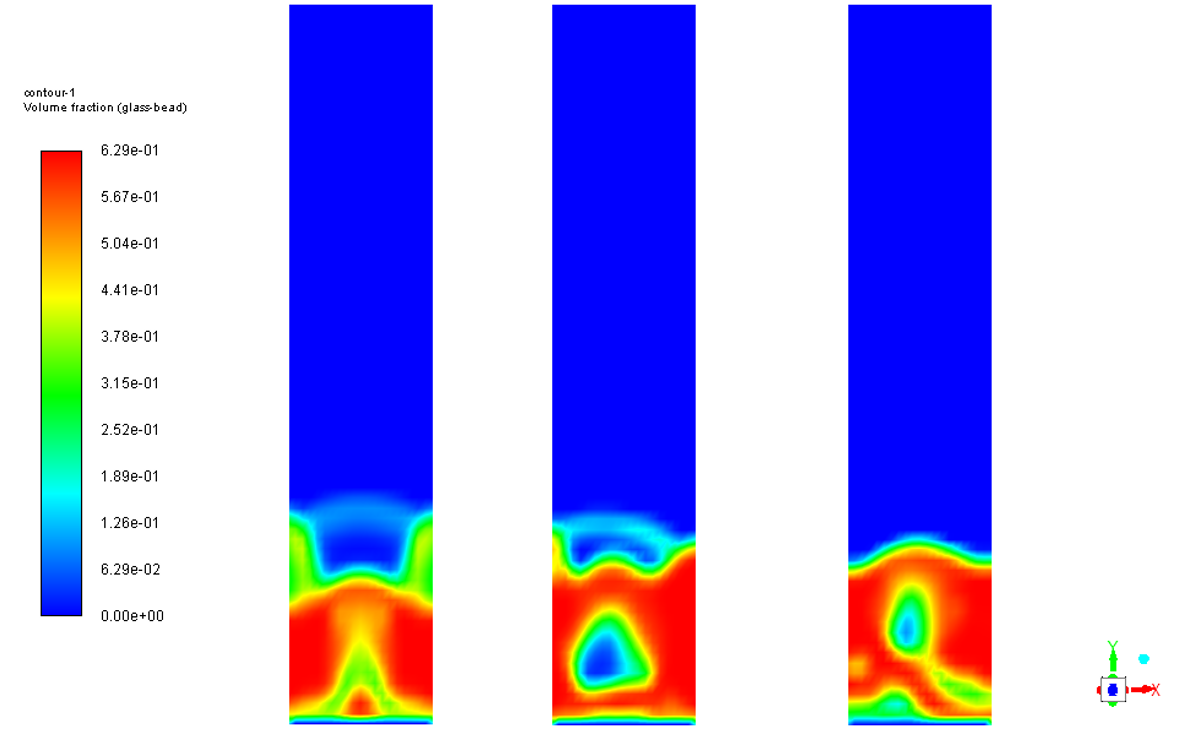
\includegraphics[width=0.9\textwidth,height=0.55\textheight,keepaspectratio]{volfrac_1_736.png} \\ % MODIFIED HEIGHT
    {\scriptsize \caption{Snapshots at t = 1s, 3s, and 5s (left to right).}}
    \vspace{0.5em}
    \begin{itemize}
        \item Observe bubble formation, rise, and eruption at the bed surface.
        \item Relatively distinct bubble shapes.
    \end{itemize}
\end{frame}

\begin{frame}{Contours: Solid Volume Fraction ($\alpha_s$) at $U_g = 2.78$ m/s}
    \frametitle{Solid Volume Fraction ($\alpha_s$) for $U_g = 2.78$ m/s}
    \centering
    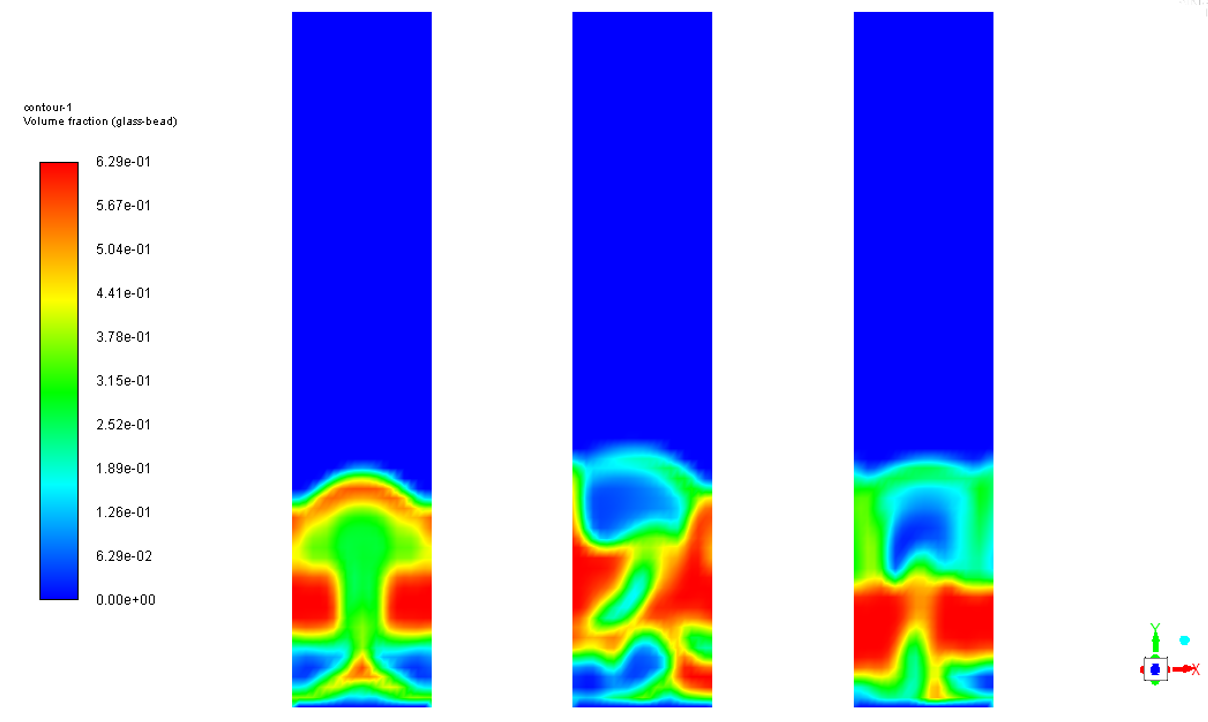
\includegraphics[width=0.9\textwidth,height=0.55\textheight,keepaspectratio]{volfrac_2_78.png} \\ % MODIFIED HEIGHT
    {\scriptsize \caption {Snapshots at t = 1s, 3s, and 5s (left to right).}}
    \vspace{0.5em}
    \begin{itemize}
        \item More vigorous bubbling, larger and more distorted bubbles.
        \item Faster bubble rise and increased solids entrainment.
        \item Suggests transition towards more turbulent fluidization.
    \end{itemize}
\end{frame}

\subsection{Contours of Solid Velocity Magnitude}
\begin{frame}{Contours: Solid Velocity Magnitude ($|\vec{U}_s|$) at $U_g = 1.736$ m/s}
    \frametitle{Solid Velocity Magnitude ($|\vec{U}_s|$) for $U_g = 1.736$ m/s}
    \centering
    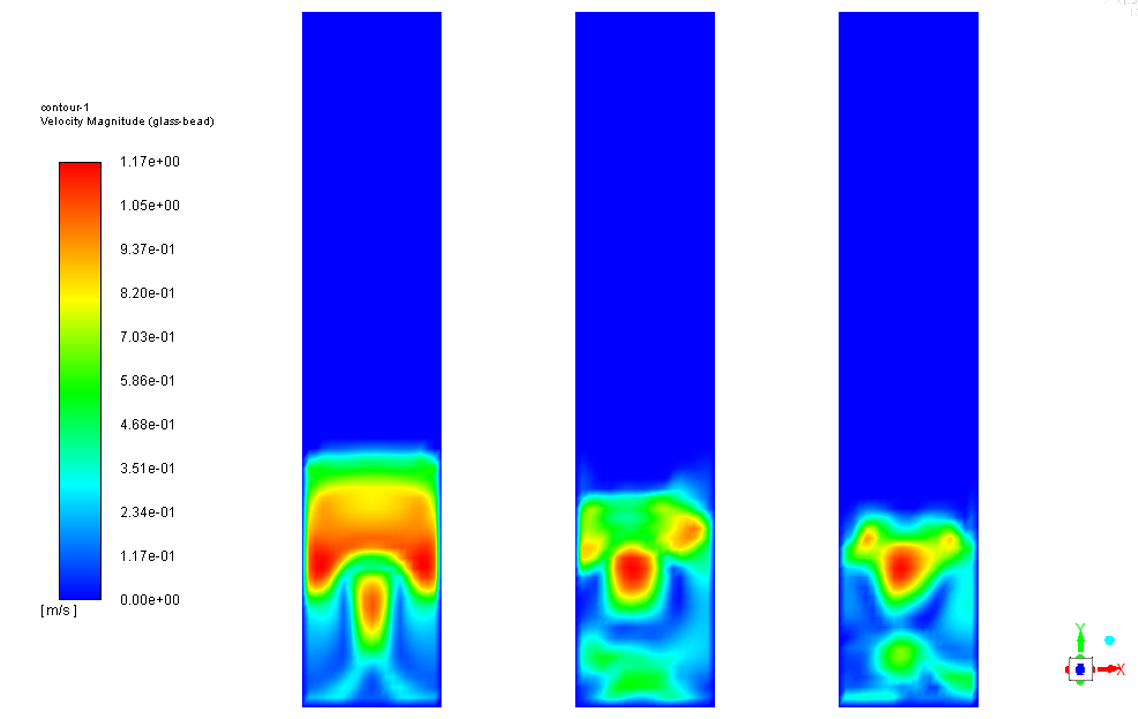
\includegraphics[width=0.9\textwidth,height=0.55\textheight,keepaspectratio]{velmag_1_736.png} \\  % MODIFIED HEIGHT
    {\scriptsize \caption {Snapshots at t = 1s, 3s, and 5s (left to right).}}
    \vspace{0.5em}
    \begin{itemize}
        \item Higher solid velocities observed in the bubble wake and near the erupting surface.
        \item Clear upward movement of solids with bubbles and downward movement near walls.
    \end{itemize}
\end{frame}

\begin{frame}{Contours: Solid Velocity Magnitude ($|\vec{U}_s|$) at $U_g = 2.78$ m/s}
    \frametitle{Solid Velocity Magnitude ($|\vec{U}_s|$) for $U_g = 2.78$ m/s}
    \centering
    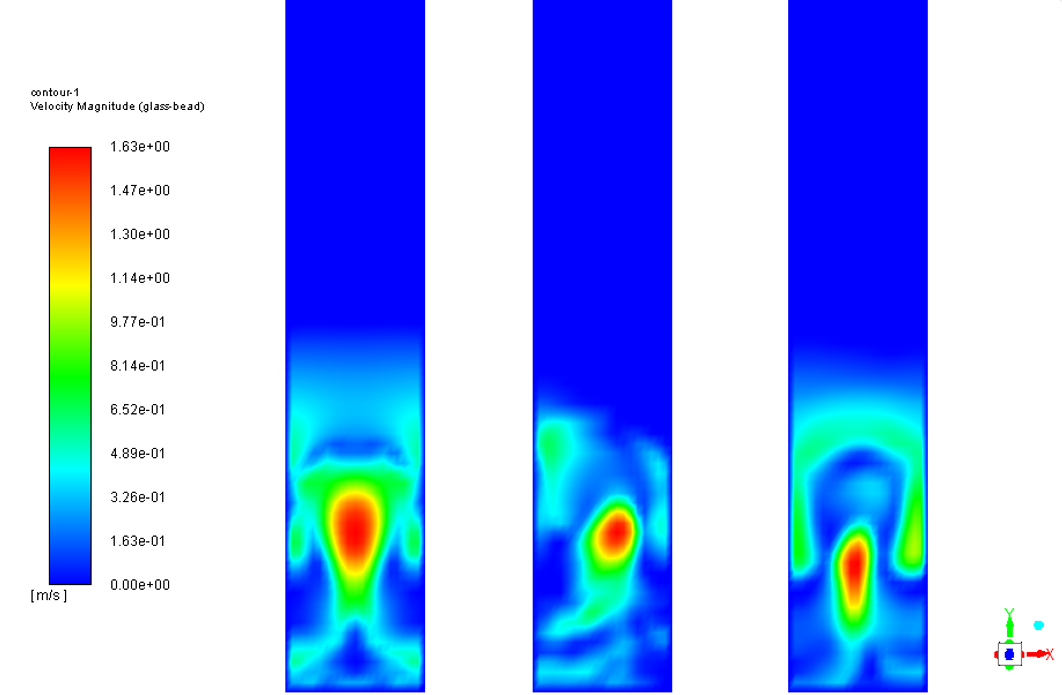
\includegraphics[width=0.9\textwidth,height=0.55\textheight,keepaspectratio]{velmag_2_78.png} \\ % MODIFIED HEIGHT
    {\scriptsize \caption {Snapshots at t = 1s, 3s, and 5s (left to right).}}
    \vspace{0.5em}
    \begin{itemize}
        \item Significantly higher peak solid velocities compared to lower $U_g$.
        \item Enhanced solid circulation and mixing throughout the bed.
    \end{itemize}
\end{frame}

\subsection{Time Evolution at Probe Location}
\begin{frame}{Time Evolution at Probe: $U_g = 1.736$ m/s}
    \frametitle{Probe Data (x=0.1, y=0.1, z=0.01m) for $U_g = 1.736$ m/s}
    \begin{columns}[T]
        \begin{column}{0.48\textwidth}
            \centering
            \textbf{Solid Velocity Magnitude} \\
            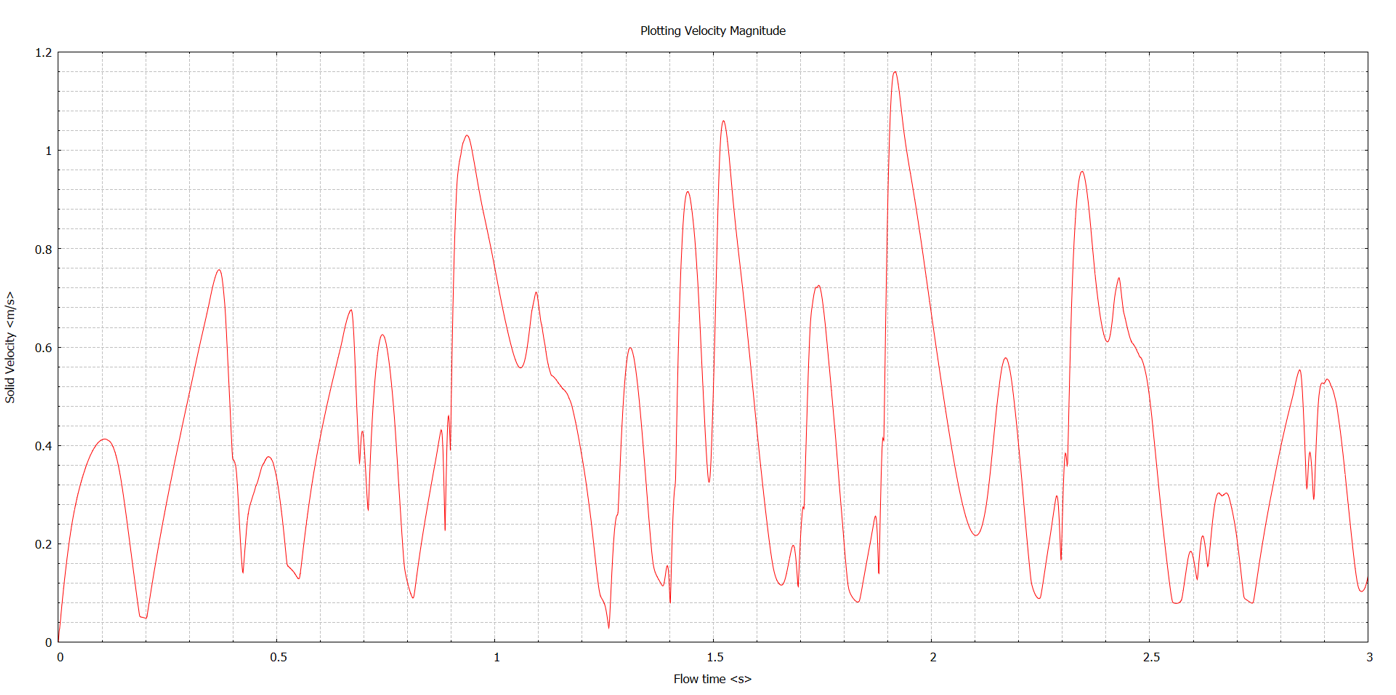
\includegraphics[width=\linewidth,height=0.4\textheight,keepaspectratio]{plot_vel_1_736.png} \\ % MODIFIED HEIGHT
            % \tiny (Report Fig. 8)
        \end{column}
        \begin{column}{0.48\textwidth}
            \centering
            \textbf{Solid Volume Fraction} \\
            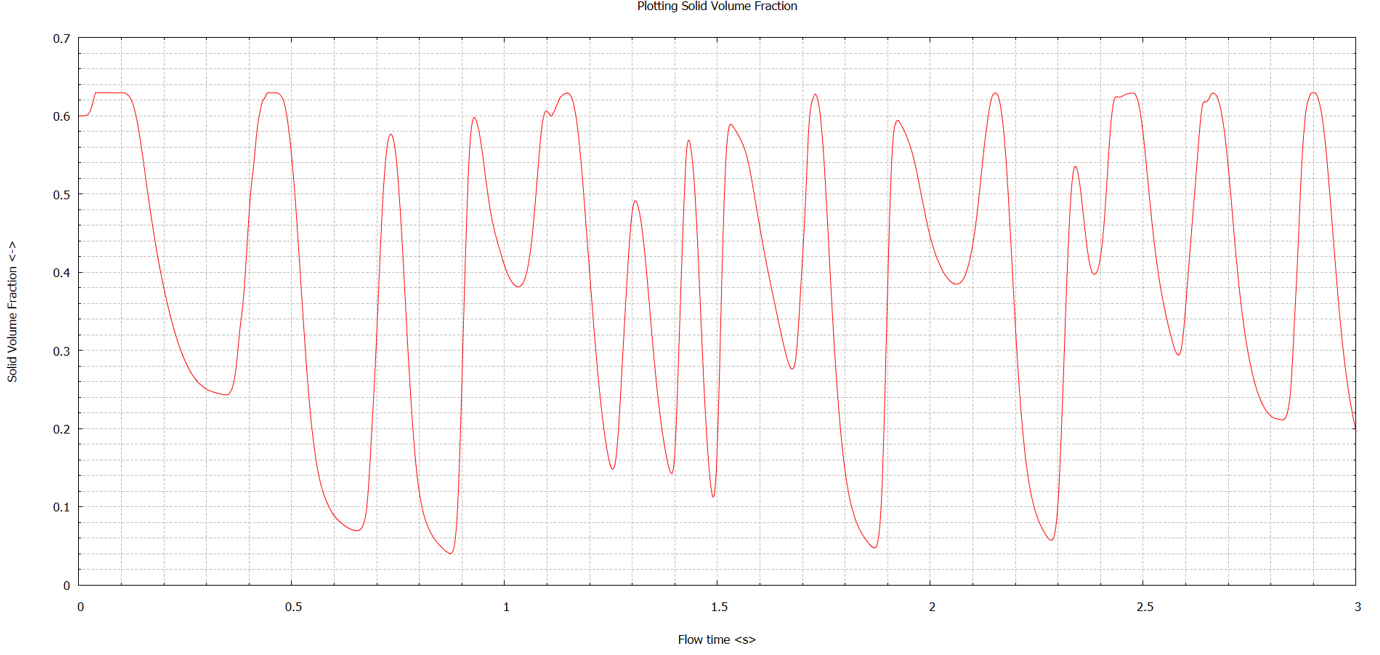
\includegraphics[width=\linewidth,height=0.4\textheight,keepaspectratio]{plot_volfrac_1_736.png} \\ % MODIFIED HEIGHT
            % \tiny (Report Fig. 9)
        \end{column}
    \end{columns}
    \begin{itemize}
        \item Fluctuations indicate passage of bubbles (low $\alpha_s$, high $|\vec{U}_s|$) and dense phase (high $\alpha_s$, low $|\vec{U}_s|$).
        \item Periodic nature reflects bubbling frequency.
    \end{itemize}
\end{frame}

\begin{frame}{Time Evolution at Probe: $U_g = 2.78$ m/s}
    \frametitle{Probe Data (x=0.1, y=0.1, z=0.01m) for $U_g = 2.78$ m/s}
    \begin{columns}[T]
        \begin{column}{0.48\textwidth}
            \centering
            \textbf{Solid Velocity Magnitude} \\
            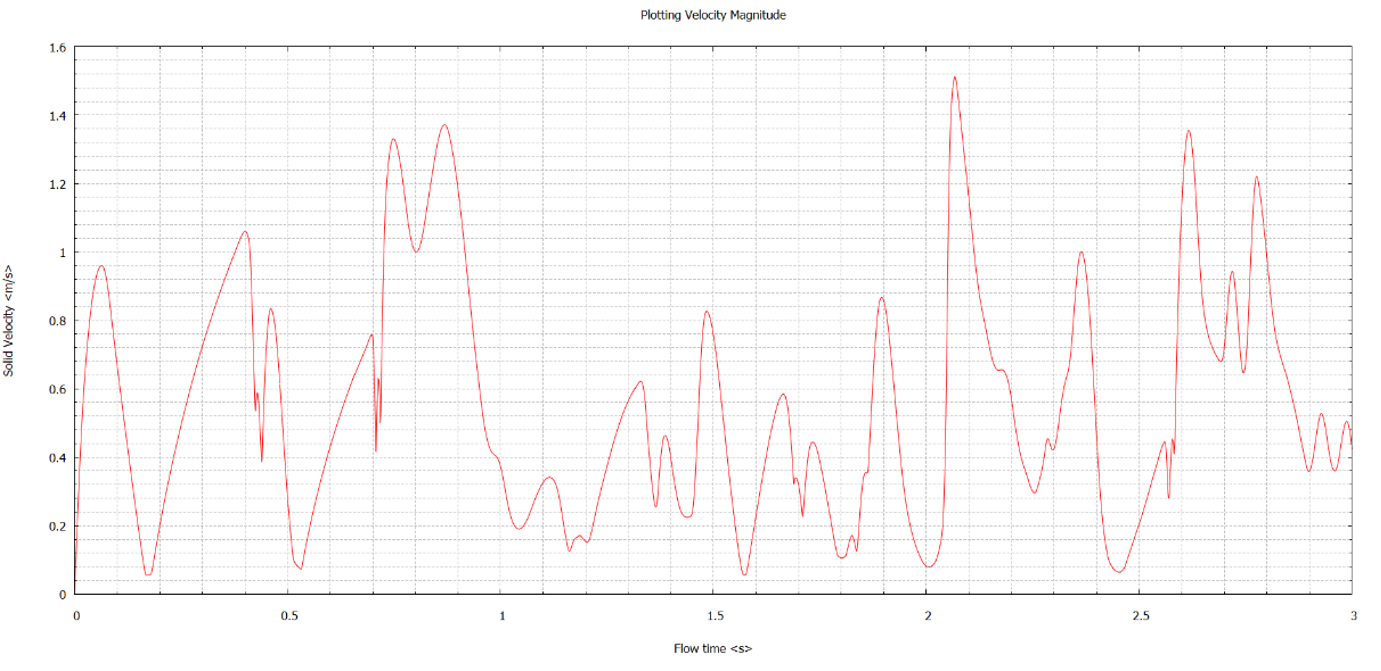
\includegraphics[width=\linewidth,height=0.4\textheight,keepaspectratio]{plot_vel_2_78.png} \\ % MODIFIED HEIGHT
            % \tiny (Report Fig. 10)
        \end{column}
        \begin{column}{0.48\textwidth}
            \centering
            \textbf{Solid Volume Fraction} \\
            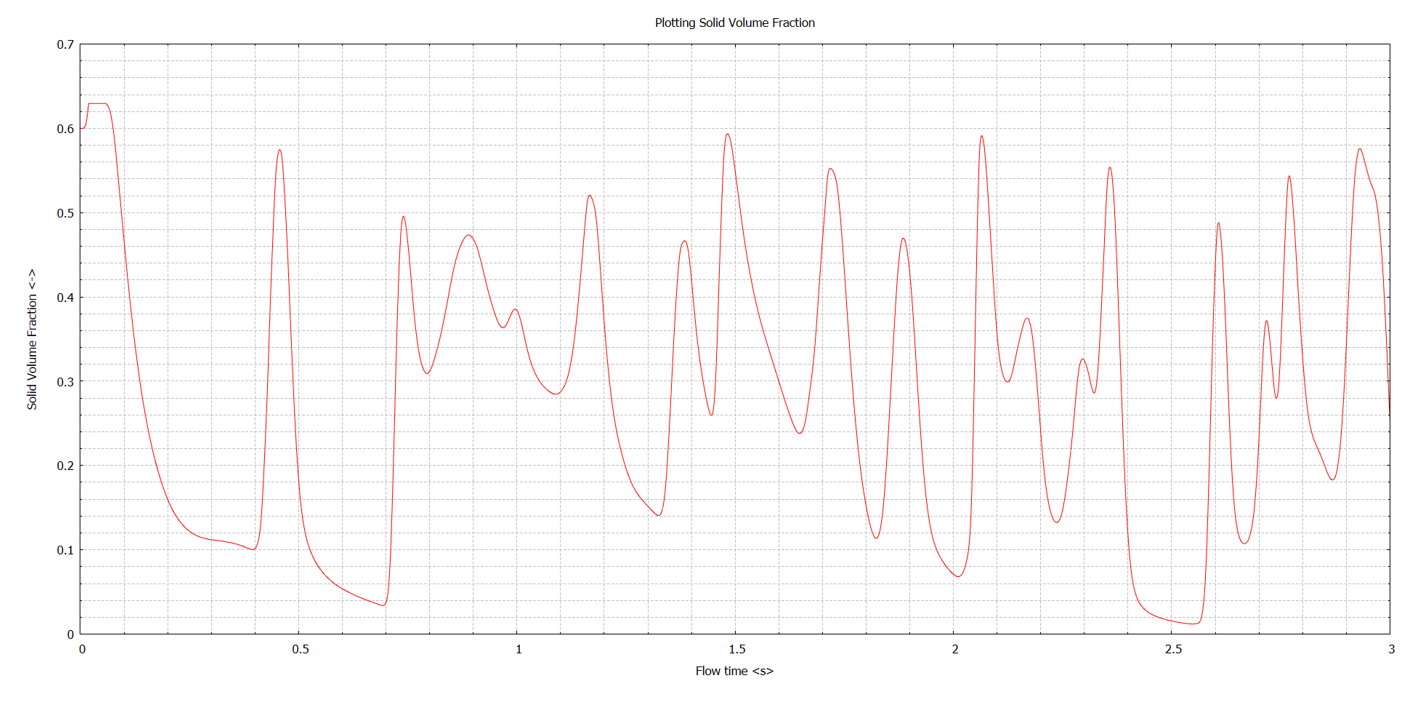
\includegraphics[width=\linewidth,height=0.4\textheight,keepaspectratio]{plot_volfrac_2_78.png} \\ % MODIFIED HEIGHT
            % \tiny (Report Fig. 11)
        \end{column}
    \end{columns}
    \begin{itemize}
        \item Sharper and more frequent peaks in velocity, deeper troughs in volume fraction.
        \item Higher peak velocities.
        \item Indicates increased bubbling frequency and intensity.
    \end{itemize}
\end{frame}

% --- OBSERVATIONS ---
\section{Key Observations}
\begin{frame}{Key Observations from Simulations}
    \textbf{Based on contours and probe data:}
    \ben
        \im \textbf{Fluctuating Solid Volume Fraction at Probe:}
            \bi
                \im Local maxima in $\alpha_s$ occur as dense phase passes.
                \im Gas pushes solids upwards (bubble passage), then solids recirculate downwards near walls and refill lower regions.
            \ei
        \im \textbf{Effect of Superficial Velocity ($U_g$):}
            \bi
                \im Higher $U_g$ (2.78 m/s) leads to increased bubbling frequency.
                \im Evident from sharper, more numerous peaks in probe data (e.g., $\alpha_s$ over 3s interval).
                \im Implies more vigorous solid recirculation.
            \ei
        \im \textbf{Bubble Morphology and Drag:}
            \bi
                \im Larger, more distorted bubbles at higher $U_g$.
                \im Increased drag force from higher gas flow contributes to this.
            \ei
        \im \textbf{Solid Velocity Distribution:}
            \bi
                \im Higher solid velocities typically seen in the upper parts of the bed and in bubble wakes.
                \im Enhanced momentum exchange between gas and solids at higher $U_g$.
            \ei
    \een
\end{frame}

% --- CONCLUSION ---
\section{Conclusion}
\begin{frame}{Conclusion}
    \ben
        \im \textbf{Model Development:}
            \bi
                \im Basic understanding of CFD simulations for fluidized beds using ANSYS Fluent (Eulerian-Eulerian TFM with KTGF) has been established.
            \ei
        \im \textbf{Preliminary Simulations \& Insights:}
            \bi
                \im Simulations of bubbling gas-solid fluidized beds performed successfully.
                \im Key phenomena like bubble formation, rise, and effect of gas velocity on bed dynamics were observed.
                \im Provides quantitative insight into bubble dynamics, particle mixing, and momentum exchange.
            \ei
    \een
    \vspace{1em}
    % \begin{block}{Significance}
    %     These findings inform optimal reactor design and scale-up strategies for industrial gas-solid processes.
    % \end{block}
\end{frame}

% --- FUTURE WORK ---
\section{Future Work}
\begin{frame}{Future Work}
    Building upon the current model and understanding:
    \ben
        \im \textbf{Detailed Single Bubble Dynamics:}
            \bi
                \im Focus on the formation, evolution, and characteristics (size, shape, velocity) of a single isolated bubble.
                \im This can involve specific injection techniques or conditions to isolate a single bubble event.
            \ei
        \im \textbf{Parametric Study for Monodispersed Systems:}
            \bi
                \im Systematically investigate the effect of particle size ($d_p$).
                \im Systematically investigate the effect of particle density ($\rho_s$).
                \im Quantify their impact on bubbling behavior (frequency, size, velocity) and overall bed hydrodynamics.
            \ei
        \im \textbf{Extension to Bi-dispersed Systems (as per original objectives):}
            \bi
                \im Investigate the effect of mixture composition (varying sizes and/or densities of particles).
                \im Study segregation and mixing patterns in bi-dispersed fluidized beds.
            \ei
        \im \textbf{Model Validation:}
            \bi
                \im Compare simulation results with experimental data from literature or dedicated experiments for quantitative validation.
            \ei
    \een
\end{frame}

% --- Q\&A ---
\begin{frame}
    \centering
    \Huge Thank You!
    \vspace{2em}
\end{frame}

\end{document}